\begin{apendicesenv}

\partapendices

\chapter{Diagramas Arquiteturais de Software}

Diagramas das arquiteturas que serão usadas nos softwares do projeto.

\begin{figure}[h]
	\center{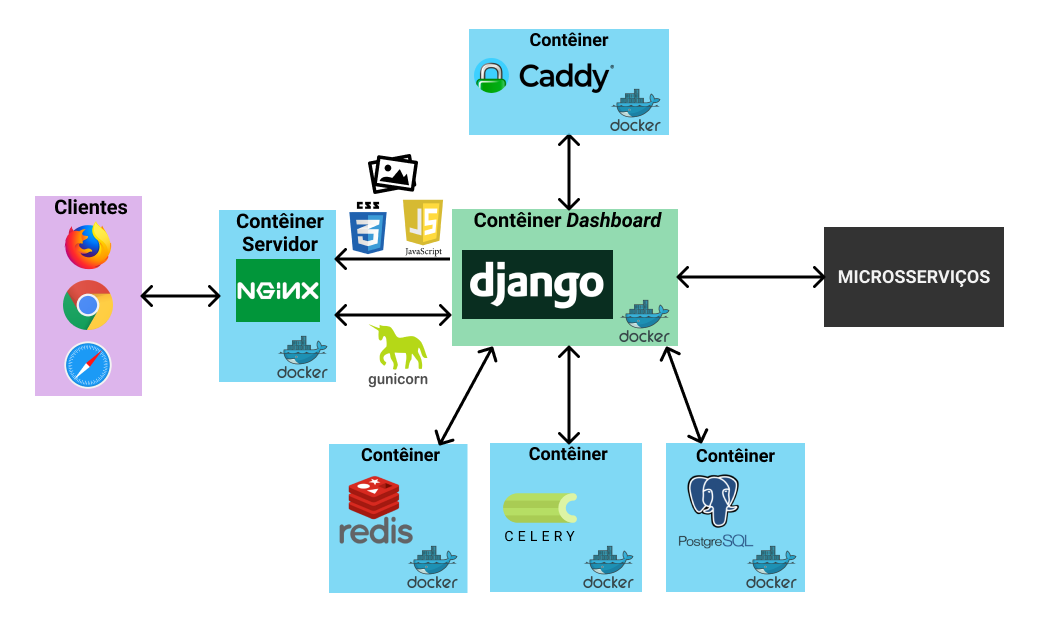
\includegraphics[width=\textwidth]{diagrama-arq-dashboard.png}}
	\caption{\label{fig:diagrama-arq-dashboard} Diagrama que mostra a arquitetura e tecnologias que serão usadas com o \textit{Dashboard}.}
\end{figure}\newpage

\begin{figure}[h]
	\center{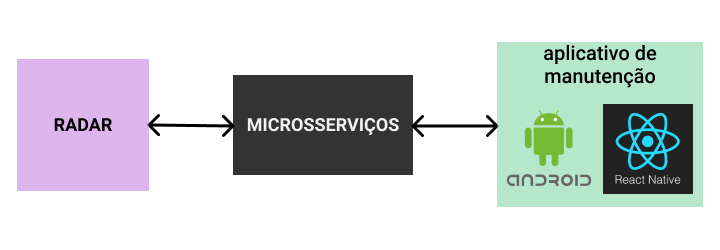
\includegraphics[width=\textwidth]{diagrama-arq-webApp.png}}
	\caption{\label{fig:diagrama-arq-webApp} Diagrama que mostra a arquitetura e tecnologias que serão usadas com o \textit{WebApp}.}
\end{figure}\newpage

\begin{figure}[h]
	\center{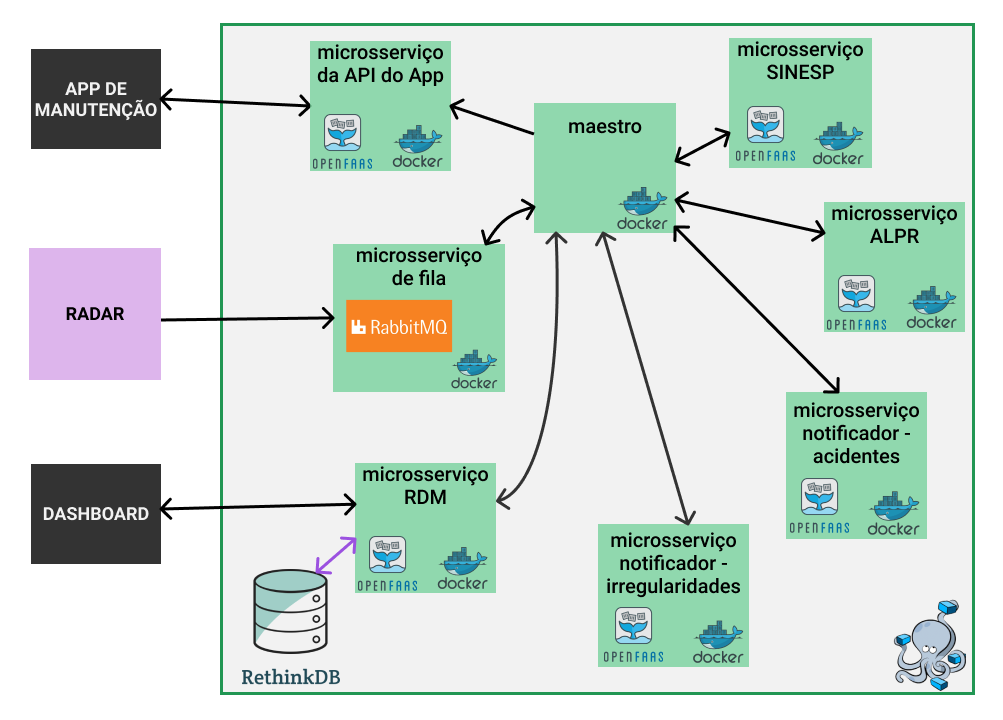
\includegraphics[width=\textwidth]{diagrama-arq-microsservicos.png}}
	\caption{\label{fig:diagrama-arq-microsservicos} Diagrama que mostra a arquitetura e tecnologias que serão usadas com os microsserviços.}
\end{figure}\newpage

\chapter{Diagrama de Comunicação dos Serviços de Software}

Diagrama que mostra como será a comunicação entre os diferentes softwares do projeto.

\begin{figure}[h]
	\center{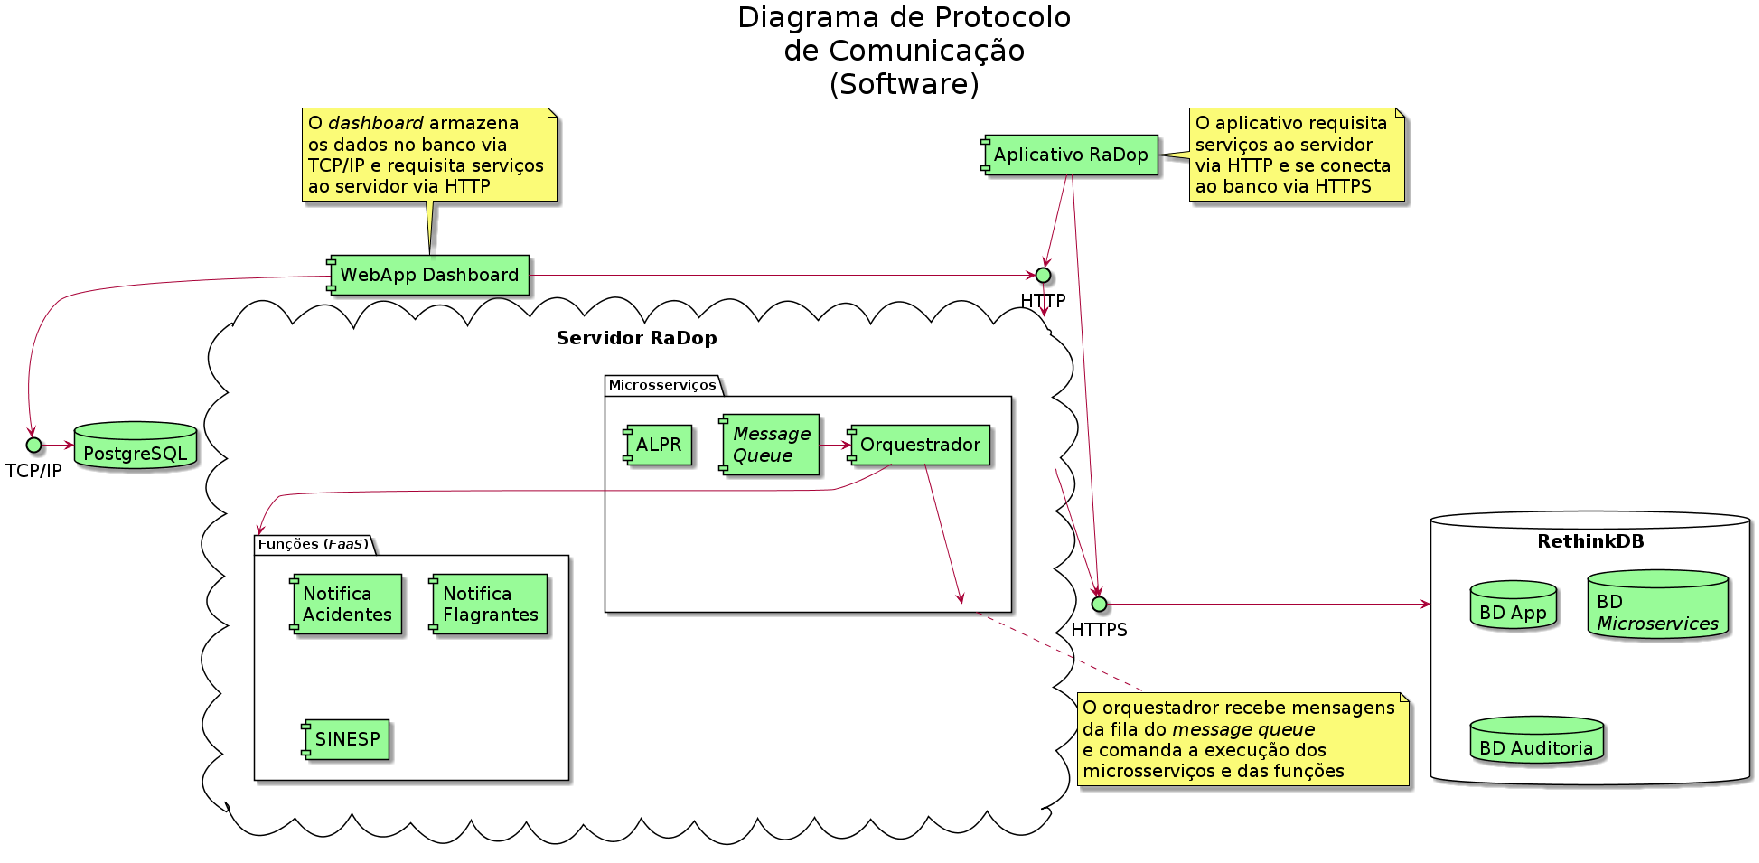
\includegraphics[width=\textwidth]{diagrama-de-comunicacao-PC2.pdf}}
	\caption{\label{fig:diagrama-comm-soft} Diagrama de comunicação dos serviços de software.}
\end{figure}

\chapter{Diagrama de Classes de Produto de Software}

Diagrama que mostra as classes que farão parte dos softwares do projeto.

\begin{figure}[h]
	\center{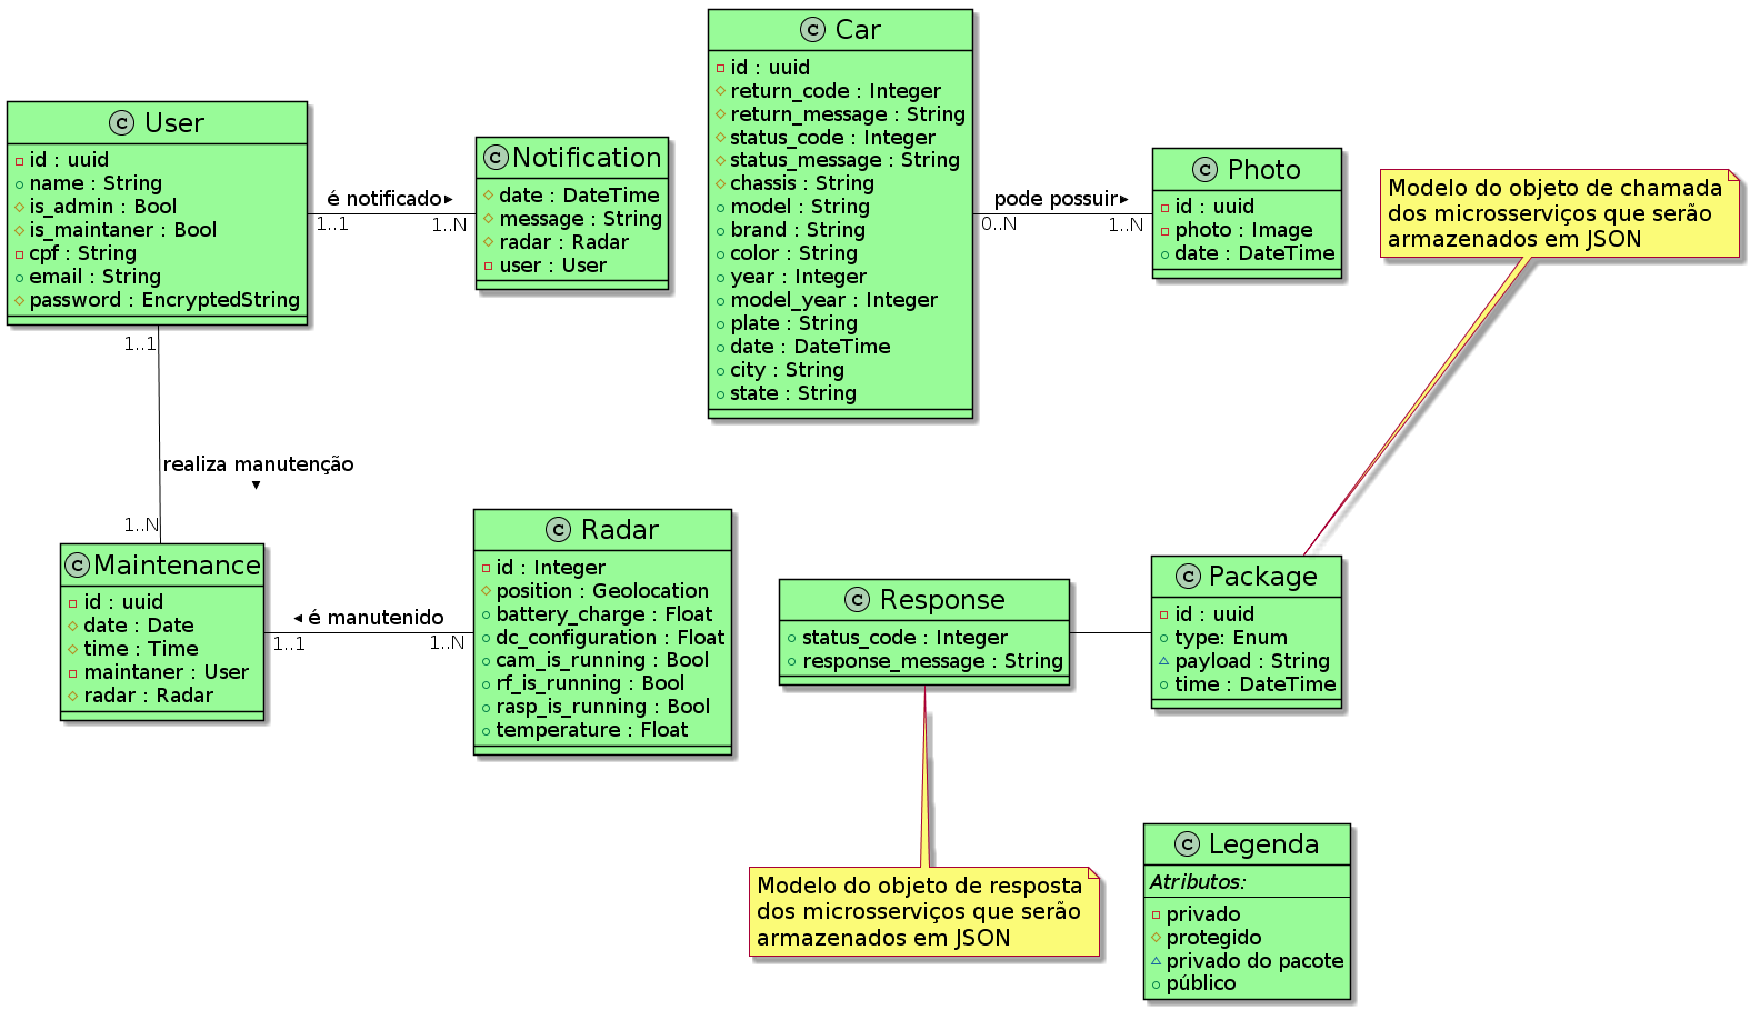
\includegraphics[scale=0.5]{diagrama-de-classes-PC2.pdf}}
	\caption{\label{fig:diagrama-classe-soft} Diagrama UML de classes dos produtos de software.}
\end{figure}

\end{apendicesenv}
